\documentclass{beamer}

\usepackage[utf8]{inputenc}
\usepackage{research}
\usepackage{IEEEtrantools}
\usepackage{ragged2e}
\usepackage[mode=buildnew]{standalone}
\usepackage{tikz}
\usepackage{nicematrix}
\usepackage{xcolor}
\usetikzlibrary{automata, positioning, arrows}


\usetheme{Copenhagen}
\usefonttheme[onlymath]{serif}

\beamertemplatenavigationsymbolsempty
\addtobeamertemplate{navigation symbols}{}{%
    \usebeamerfont{footline}%
    \usebeamercolor[fg]{footline}%
    \hspace{1em}%
    \insertframenumber/\inserttotalframenumber
}

\title{Research Meeting}
\author{Hugo Aguettaz}
\institute{Institut für Signal- und Informationsverarbeitung\\ETH Zürich}
\date{\today}



\begin{document}
	\begin{frame}
		\titlepage
	\end{frame} 

	\begin{frame}{PhD course plan}
		12 ECTS are required :
		\begin{itemize}
			\item Deep Learning in Artificial and Biological Neuronal Networks (4 ECTS) : done!
			\item Algebra and Error Correcting Codes (6 ECTS) : Spring 2022
			\item Learning to Teach (2 ECTS) : Fall 2022
		\end{itemize}
	\end{frame} 

	\begin{frame}{Erratum}{Dale's Principle}
		\justifying
		\begin{block}{\emph{Encyclopaedia Britannica}}
			\justifying
			\emph{"[Sir Henry Dale] stated that a neurotransmitter releases at one axon terminal of a neuron can be presumed to be released at other axon terminals of the same neuron. Dale's principle refers only to he presynaptic neuron, as the responses of different postsynaptic receptors to a single neurotransmitter can vary in the same or different neurons."}
		\end{block}
		\begin{block}{\emph{Principles of Neural Science, Sixth Edition} by Kandel et al.}
			\justifying
			\emph{"There are two major classes of transmitters receptors. Ionotropic receptors are ligand-gated ion channels. Binding of transmitter to an extracellular binding site triggers a conformational change that opens the channel pore, generating an ionic current that excites (depolarizes) or inhibits (hyperpolarizes) the postsynaptic cells, depending on the receptor."}
		\end{block}
	\end{frame}

	\begin{frame}{Recurrent Spiking Neural Networks}{Memorization}
		\justifying
		\begin{block}{Conjecture}
			\justifying
			A RSNN with $N > 0$ neurons and a causal impulse response $h$ with (finite) duration $T_h > 0$, is able to memorize any sequence in $\mathcal{M}_{L, Tr, Th}^N$.
		\end{block}
	\end{frame}

	\begin{frame}{Firing sequences}{Single channel}
		\justifying
		\begin{definition}[Firing sequence - single channel]
			\justifying
			A (single channel) firing sequence with length $L > 0$ and refractory period $T_r \geq 0$ is a binary sequence with at least $T_r$ zeros between two consecutifs ones, including between the last one and the first one of the sequence.
		\end{definition}

		We denote by $\set{F}_{L, T_r}$ the set of all (single-channel) firing sequences with length $L$ and refractory period $T_r$. 
		We can also define the set of all (single-channel) firing sequences with length $L$ and refractory period $T_r$, where we relax the constraint on the minimum number of zeros between the last one and the first one of the sequence. We denote this set by $\set{\tilde{F}}_{L, T_r}$. 

		% \begin{example}
		% 	\justifying
		% 	$(0, 0, 0, 0, 0, 0, 0)$ and $(0, 1, 0, 0, 1, 0, 0)$ are (single-channel) firing sequences with refractory period $2$ and length $7$ but $(1, 1, 1, 1, 1, 1, 1)$ and $(1, 0, 0, 1, 0, 0, 1)$ are not.
		% \end{example}
	\end{frame}

	\begin{frame}{Intermezzio}{Generalized golden ratio}
		\justifying
		\begin{definition}[Generalized golden ratio]
			\justifying
			Let $P(x) := x^p - x^{p-1} - 1$ with $p > 0$. The roots of $P(x)$ are denoted by $\varphi_{p, i}$ for $i = 1, \dots, p$. Moreover, we call generalized golden ratio and denote it by $\hat{\varphi}_p$ the root with the greatest modulus.
		\end{definition}
		
		\begin{table}
			\centering
			\begin{tabular}{*{8}{c}}
				\toprule
				$p$ & $\hat{\varphi}_p$ & $p$ & $\hat{\varphi}_p$ & $p$ & $\hat{\varphi}_p$ & $p$ & $\hat{\varphi}_p$ \\
				\midrule
				1 & 2 & 6 & 1.285199 & 11 & 1.184276 & 16 & 1.140034 \\
				2 & 1.618034 & 7 & 1.255423 & 12 & 1.172951 & 17 & 1.133902 \\
				3 & 1.465571 & 8 & 1.232055 & 13 & 1.163120 & 18 & 1.128356 \\
				4 & 1.380278 & 9 & 1.213150 & 14 & 1.154494 & 19 & 1.123311 \\
				5 & 1.324718 & 10 & 1.197491 & 15 & 1.146854 & 20 & 1.118699 \\
				\bottomrule
			\end{tabular}
		\end{table}

		One can show that for any $p > 0$, $\hat{\varphi}_p$ is real and in the range $(1, 2]$.
	\end{frame}


	\begin{frame}{Firing sequences}{Single channel}
		\begin{theorem}[Cardinality]
			\justifying
			The cardinality of $\set{F}_{L, T_r}$ is given by:
			\begin{equation*}
				\card{\set{F}_{L, T_r}} = \sum_{i = 1}^{T_r + 1} \varphi_{T_r + 1, i}^L,
			\end{equation*}
			where $\varphi_{T_r + 1, i}$ for $i = 1, \dots, T_r + 1$ are the roots of $P(x) := x^{T_r + 1} - x^{T_r} - 1$.
		\end{theorem}
		\justifying
		It follows that 
		\begin{equation*}
			\lim_{L \to \infty} \card{\set{F}_{L, T_r}} = \hat{\varphi}_{T_r + 1}^L,
		\end{equation*}
		where $\hat{\varphi}_{T_r + 1}$ is the generalized golden ratio of order $T_r + 1$ as defined before. Moreover, for $L \gg T_r$, $\hat{\varphi}_{T_r + 1}^L$ is actually an excellent approximate for $\card{\set{F}_{L, T_r}}$.

	\end{frame}

	\begin{frame}{Firing sequences}{Single channel}
		\begin{proofs}[\proofname \ (1/4)]
			\justifying
			For $k = 0, \dots, L-1$, we define
			\begin{equation*}
				Z_k := (X_{k-T_r}, \dots, X_k) \in \set{\tilde{F}}_{T_r + 1, T_r}
			\end{equation*}
			and 
			\begin{equation*}
				g_{k, k+1}(z_k, z_{k+1}) := \Indicator{x_{k-T_r}, \dots, x_{k+1} \in \set{\tilde{F}}_{T_r + 2, T_r}} = g(z_k, z_{k+1}),
			\end{equation*}
			where all indices are taken modulo $L$, and we draw the following factor graph.

			\begin{figure}[!ht]
				\centering
				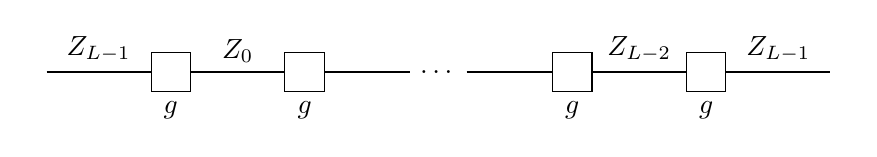
\begin{tikzpicture}[node distance={17mm}] 
					\tikzstyle{box} = [draw, rectangle, minimum width=5mm, minimum height=5mm]
					\node (1) {};
					\node[box] (2) [right of=1] [label=below:$g$] {}; 
					\node[box] (3) [right of=2] [label=below:$g$] {}; 
					\node (4) [right of=3] {$\dots$}; 
					\node[box] (5) [right of=4] [label=below:$g$] {}; 
					\node[box] (6) [right of=5] [label=below:$g$] {}; 
					\node (7) [right of=6] {};
					\draw (1) -- node[above] {$Z_{L-1}$} (2);
					\draw (2) -- node[above] {$Z_0$} (3);
					\draw (3) -- (4);
					\draw (4) -- (5);
					\draw (5) -- node[above] {$Z_{L-2}$} (6);
					\draw (6) -- node[above] {$Z_{L-1}$} (7);
				\end{tikzpicture}
			\end{figure}
		\end{proofs} 
	\end{frame}

	% \begin{frame}{Firing sequences}{Single channel}
	% 	\begin{proofs}[\proofname \ (2/4)]
	% 		\justifying
	% 		With $Z_L = \breve{z}_L$ (arbitrary but fixed), we obtain the \emph{free-loop} factor graph drawn below:

	% 		\begin{figure}[!ht]
	% 			\centering
	% 			\begin{tikzpicture}[node distance={16mm}] 
	% 				\tikzstyle{fix} = [draw, fill=black, rectangle, minimum width=3mm, minimum height = 3mm]
	% 				\tikzstyle{box} = [draw, rectangle, minimum width=5mm, minimum height=5mm]
	% 				\node[fix] (1) [label=above:$\breve{z}_L$] {};
	% 				\node[box] (2) [right of=1] [label=below:$g$] {}; 
	% 				\node[box] (3) [right of=2] [label=below:$g$] {}; 
	% 				\node (4) [right of=3] {$\dots$}; 
	% 				\node[box] (5) [right of=4] [label=below:$g$] {}; 
	% 				\node[box] (6) [right of=5] [label=below:$g$] {}; 
	% 				\node[fix] (7) [right of=6] [label=above:$\breve{z}_L$] {};
	% 				\draw (1) -- node[above] {$Z_L$} (2);
	% 				\draw (2) -- node[above] {$Z_1$} (3);
	% 				\draw (3) -- (4);
	% 				\draw (4) -- (5);
	% 				\draw (5) -- node[above] {$Z_{L-1}$} (6);
	% 				\draw (6) -- node[above] {$Z_{L}$} (7);
	% 			\end{tikzpicture}
	% 		\end{figure}

	% 		Thus, we can compute the partition of the original factor graph by sum-product message passing:
	% 		\begin{equation*}
	% 			\card{\set{F}_{L, T_r}} = \sum_{\breve{z}_L} \msgf{\mu}{Z_L}(\breve{z}_L) \msgb{\mu}{Z_L}(\breve{z}_L).
	% 		\end{equation*}
	% 	\end{proofs} 
	% \end{frame}

	\begin{frame}{Firing sequences}{Single channel}
		\begin{proofs}[\proofname \ (2/4)]
			\justifying
			For any $k = 1, \dots, L$, $Z_k$ only takes values in:
			\begin{equation*}
				\set{\tilde{F}}_{T_r + 1, T_r} = \{\overbrace{0}^{\text{1st el.}}, \overbrace{\vec{e_1}}^{\text{2nd el.}}, \overbrace{\vec{e_2}}^{\text{3rd el.}}, \dots, \overbrace{\vec{e_{T_r}}}^{T_r + 1\text{-th el.}}, \overbrace{\vec{e_{T_r + 1}}}^{T_r + 2\text{-th el.}}\},
			\end{equation*} 
			with 
			\begin{equation*}
				\vec{0} := \trans{[\overbrace{0, \cdots, 0}^{T_r + 1}]} \text{ and } \vec{e_i} := \trans{[\overbrace{0, \cdots, 0}^{i-1}, 1, \overbrace{0, \cdots, 0}^{T_r + 1 - i}]}.
			\end{equation*} 
			We express the messages in vector notation using the same ordering, i.e., 1st element corresponds to $\vec{0}$, 2nd element to $\vec{e_1}$, 3rd element to $\vec{e_2}$, and so on.
		\end{proofs} 
	\end{frame}

	\begin{frame}{Firing sequences}{Single channel}
		\begin{proofs}[\proofname \ (3/4)]
			\justifying
			The sum-product message passing can be expressed in matrix form:
			\begin{equation*}
				\vec{\msgb{\mu}{Z_k}} = \vec{\msgb{\mu}{Z_{k + 1}}} \mat{A} \text { with }
				\mat{A} = 
				\begin{bNiceArray}{ccccc}[margin] 
					1 & \Block{4-4}{\mat{I_{T_r + 1}}} \\
					0 & & & & \\
					\Vdots & & & & \\
					0 & & & & \\
					1 & 1 & 0 & \Cdots & 0\\
				\end{bNiceArray}.
			\end{equation*} 

			One can notice that the partition sum of the graph is then given by:
			\begin{equation*}
				\card{\set{F}_{L, T_r}} = \trace{\mat{A}^L}.
			\end{equation*}
		\end{proofs} 
	\end{frame}

	\begin{frame}{Firing sequences}{Single channel}
		\begin{proof}[\proofname \ (4/4)]
			\justifying
			By inspection on $\mat{A}$, one can determine its characteristic polynomial:
			\begin{equation*}
				P_A(x) = x (x^{T_r + 1} - x^{T_r} - 1) = x \prod_{i = 1}^{T_r + 1} (x - \varphi_{T_r + 1, i})
			\end{equation*}
			whose roots are the eigenvalues of $\mat{A}$. The result is now obvious as 
			\begin{equation*}
				\trace{\mat{A}^L} =  \sum_{i = 1}^{T_r + 1} \varphi_{T_r + 1, i}^L.
			\end{equation*}
		\end{proof} 
	\end{frame}

	\begin{frame}{Firing sequences}{Multiple channels}
		\justifying
		\begin{definition}[Firing sequence - multiple channels]
			\justifying
			An $N$-channels firing sequence with length $L > 0$ and refractory period $T_r \geq 0$ is a $N$-dimensional binary sequence such that each channel is a single-channel firing sequence with length $L$ and refractory period $T_r$.
		  \end{definition}

		  We denote by $\set{F}_{L, T_r}^N$ the set of all $N$-dimensional firing sequence with length $L$ and refractory period $T_r$.

		\begin{theorem}[Cardinality]
			\justifying
			The cardinality of $\set{F}_{L, T_r}^N$ is given by 
			\begin{equation*}
				\card{\set{F}_{L, T_r}^N} = \card{\set{F}_{L, T_r}}^N.
			\end{equation*}
		  \end{theorem}
	\end{frame}

	\begin{frame}{Firing sequences}{Predictability}
		\justifying
		\begin{definition}[Predictable firing sequence]
			\justifying
			Let $L > 0$ and $T_w > T_r \geq 0$. An $N$-channels firing sequence $\mat{f^N} = (\vec{f_0^N}, \vec{f_1^N}, \dots, \vec{f_{L-1}^N}) \in \set{F}_{L, T_r}^N$ is said $T_w$ predictable, if $\vec{f_k^N}$ is fully determined by $(\vec{f_{k-T_w}^N}, \dots, \vec{f_{k-1}^N})$, for any $0 \leq k < L$.
		\end{definition}

		We denote by $\set{P}_{L, T_r, T_w}^N$ the set of all $N$-dimensional $T_W$-predictable firing sequences.
	\end{frame}

	\begin{frame}{Firing sequences}{Predictability}
		\begin{example}
			
			\justifying
			With $L = 12$, $T_r = 2$, $N = 2$, and $T_w = 4$, we consider the following firing sequences :
			\begin{equation*}
				\mat{f_1} = 
				\begin{bmatrix}
					0 & 1 & 0 & 0 & {\color{purple} 0} & 1 & 0 & 0 & {\color{purple} 1} & 0 & 0 & 0 \\ 
					0 & 0 & 1 & 0 & {\color{purple} 0} & 0 & 1 & 0 & {\color{purple} 0} & 0 & 1 & 0 \\ 
				\end{bmatrix},
			\end{equation*}
			\begin{equation*}
				\mat{f_2} = 
				\begin{bmatrix}
					0 & 0 & 0 & 0 & 1 & 0 & 0 & 0 & 1 & 0 & 0 & 1 \\ 
					0 & 0 & 0 & 0 & 0 & 0 & 1 & 0 & 0 & 1 & 0 & 0 \\ 
				\end{bmatrix},
			\end{equation*}
			and
			\begin{equation*}
				\mat{f_3} = 
				\begin{bmatrix}
					0 & 1 & 0 & 0 & 0 & 1 & 0 & 0 & 0 & 1 & 0 & 0 \\ 
					0 & 0 & 1 & 0 & 0 & 0 & 1 & 0 & 0 & 0 & 1 & 0 \\ 
				\end{bmatrix}.
			\end{equation*}
			$\mat{f_1}$ is not $T_w$-predictable but $\mat{f_2}$ and $\mat{f_3}$ are.
		\end{example}
	\end{frame}

	\begin{frame}{Finite State Machine}
		\justifying
		It is obvious that any predictable sequence can be stored by an FSM. Basically, starting from any $T_w$-window of such a sequence, on can perfectly reconstruct it by following the transition of the FSM. 

		\begin{example}
			\justifying
			With $N=2$, $L=4$, and $T_r=1$, let's consider the sequence
			\begin{equation*}
				\mat{f} = 
				\begin{bNiceArray}{cccc}[margin] 
					0 & 1 & 0 & 1 \\ 
					1 & 0 & 0 & 0 \\ 
				\end{bNiceArray} \in \set{F}_{L, T_r}^N
			\end{equation*}
			For $T_w = 1$, this sequence is obviously not $T_w$-predictable since the window $\begin{bmatrix} 1 \\ 0 \end{bmatrix}$ can be followed either by $\begin{bmatrix} 0 \\ 0 \end{bmatrix}$, either by $\begin{bmatrix} 0 \\ 1 \end{bmatrix}$. For $T_w = 2$, it is predictable and we can construct the FSM of this sequence.
		\end{example}
	\end{frame}

	\begin{frame}{Finite State Machine}
		\begin{example}
			\justifying
			\begin{table}
				\centering
				\begin{tabular}{c c c}
					\toprule
					Current state & Next state & Output \\
					\midrule
					$\begin{bmatrix} 0 & 1 \\ 1 & 0 \end{bmatrix}$ & $\begin{bmatrix} 1 & 0 \\ 0 & 0 \end{bmatrix}$ & $\begin{bmatrix} 0 \\ 1 \end{bmatrix}$ \\
					$\begin{bmatrix} 1 & 0 \\ 0 & 0 \end{bmatrix}$ & $\begin{bmatrix} 0 & 1 \\ 0 & 0 \end{bmatrix}$ & $\begin{bmatrix} 1 \\ 0 \end{bmatrix}$ \\
					$\begin{bmatrix} 0 & 1 \\ 0 & 0 \end{bmatrix}$ & $\begin{bmatrix} 1 & 0 \\ 0 & 1 \end{bmatrix}$ & $\begin{bmatrix} 0 \\ 0 \end{bmatrix}$ \\
					$\begin{bmatrix} 1 & 0 \\ 0 & 1 \end{bmatrix}$ & $\begin{bmatrix} 0 & 1 \\ 1 & 0 \end{bmatrix}$ & $\begin{bmatrix} 1 \\ 0 \end{bmatrix}$ \\
					\bottomrule
				\end{tabular}
			\end{table}

			Starting from any state, one can perfectly reproduce a periodic extension of the sequence.
		\end{example}
	\end{frame}

	\begin{frame}{Firing sequences}{Predictability}
		\justifying
		For any $N > 0$, $L > 0$ and $T_r \geq 0$, we would like to determine the lowest $T_w > T_r$ such that, for any arbitrarily small $\varepsilon > 0$, we have
		\begin{equation*}
			p := \Pr{\mat{f} \in \set{P}_{L, T_r, T_w}^N | \mat{f} \in \set{F}_{L, T_r}^N} \geq 1 - \varepsilon
		\end{equation*}

		Computing this probability is the same as computing the cardinality of $\set{F}_{L, T_r}^N \setminus \set{P}_{L, T_r, T_w}^N$. Finding a closed-form expression is out of the scope of our work. However, one can observe that $p$ increases exponentially with both $T_w$ and $N$ but decreases with $L$ and $T_r$.
	\end{frame}

	\begin{frame}{Firing sequences}{Predictability}
		\justifying
		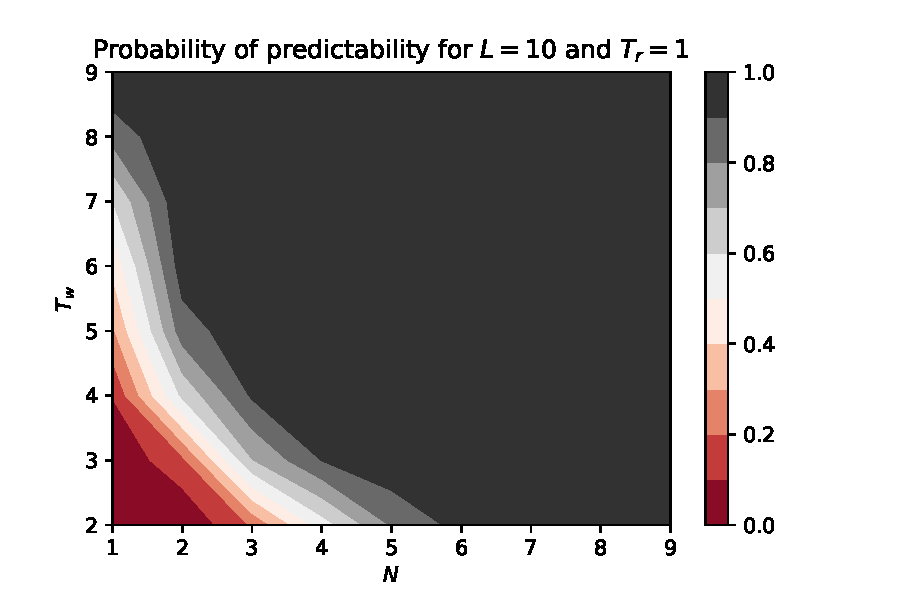
\includegraphics[width=\textwidth]{predictability_10_1.pdf}
	\end{frame}

	\begin{frame}{Firing sequences}{Predictability}
		\justifying
		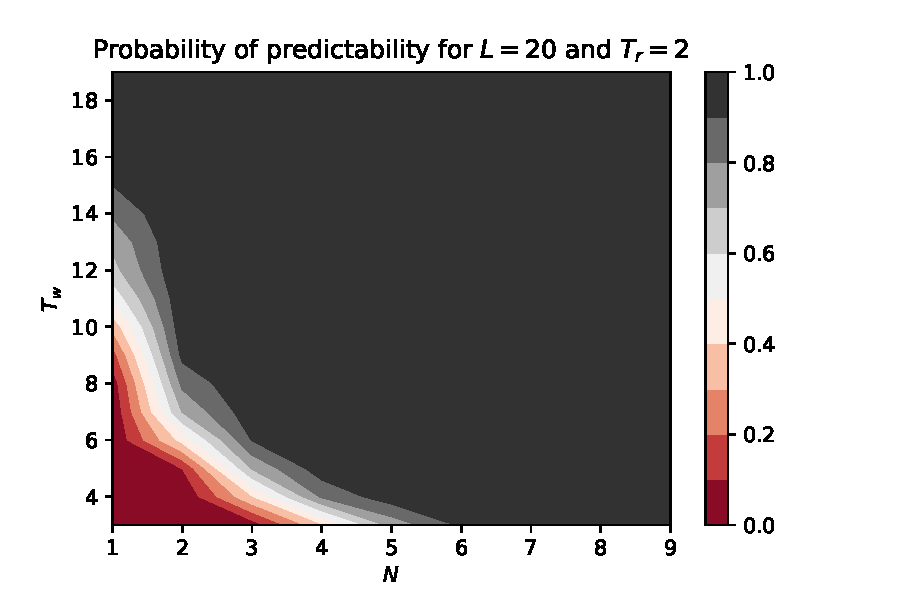
\includegraphics[width=\textwidth]{predictability_20_2.pdf}
	\end{frame}


	% \begin{frame}{Firing sequences}{Reducibility}
	% 	\justifying
	% 	\begin{definition}[Reducible firing sequence]
	% 		\justifying
	% 		An $N$-channels firing sequence with length $L > 0$ and refractory period $T_r \geq 0$ is said $T_d$ reducible if it is $T_d$-periodic, with $T_d < L$.
	% 	\end{definition}

	% 	We denote by $\set{D}_{L, T_r, T_d}^N$ the set of all $N$-dimensional $T_d$-reducible firing sequence with length $L$ and refractory period $T_r$.
	% \end{frame}

	% \begin{frame}{Firing sequences}{Reducibility}
	% 	\justifying
	% 	\begin{theorem}
	% 		\justifying
	% 		Let $L, T_d > 0$ and define $\tilde{T}_d := \gcd (L, T_d)$. We have
	% 		\begin{equation*}
	% 			\set{D}_{L, T_r, T_d}^N = \set{D}_{L, T_r, \tilde{T}_d}^N.
	% 		\end{equation*}
	% 	\end{theorem}
	% 	\begin{corollary}[Cardinality]
	% 		\justifying
	% 		The cardinality  of $\set{D}_{L, T_r, T_d}^N$ is given by:
	% 		\begin{equation*}
	% 			\card{\set{D}_{L, T_r, T_d}^N} = \card{\set{F}_{\tilde{T}_d, T_r}^N},
	% 		\end{equation*}
	% 		with $\tilde{T}_d = \gcd (L, T_d)$.
	% 	\end{corollary}
	% \end{frame}

	% \begin{frame}{Firing sequences}{Redundancy}
	% 	\justifying
	% 	\begin{definition}[Redundant firing sequence]
	% 		\justifying
	% 		An $N$-channels firing sequence with length $L > 0$ and refractory period $T_r \geq 0$ is said $T_c$-redudant if it contains at least two identical $N$-channels subsections of length $T_c$.
	% 	\end{definition}

	% 	We denote by $\set{C}_{L, T_r, T_c}^N$ the set of all $T_c$-redundant firing sequences with length $L$ and refractory period $T_r$.
	% \end{frame}

	% \begin{frame}{Firing sequences}{Memorizability}
	% 	\justifying
	% 	\begin{definition}[Memorizable firing sequence]
	% 		\justifying
	% 		An $N$-channels firing sequence with length $L > 0$ and refractory period $T_r \geq 0$ is said $T_w$-memorizable if all identical $N$-channels subsections of length $T_w$ are followed by the same $N$-dimensional binary vector.
	% 	\end{definition}

	% 	We denote by $\set{M}_{L, T_r, T_w}^N$ the set of all $N$-dimensional $T_w$-memorizable firing sequences with length $L$, refractory period $T_r$, and working memory $T_w$.
	% 	% \begin{example}
	% 	% 	\justifying
	% 	% 	$(0, 1, 0, 0, 1, 0, 0)$ and $(0, 0, 0, 0, 0, 0, 0)$ are $4$-reasonable but $(0, 0, 0, 0, 0, 1, 0)$ is not.
	% 	% \end{example}
	% \end{frame}

	\begin{frame}{Firing sequences}{Examples}
		\justifying
		Let $L = 10$, $T_r = 2$, $N = 2$, and $T_w = T_c = T_d = 5$.
		\begin{itemize}
			\justifying
			\item 
				$\mat{f_1} = 
				\begin{bNiceArray}{cccccccccc}[margin] 
					0 & 1 & 0 & 0 & 0 & 0 & 1 & 0 & 0 & 0 \\ 
					0 & 0 & 1 & 0 & 0 & 0 & 0 & 1 & 0 & 0 \\ 
				\end{bNiceArray}$
			is a 2 channels firing sequence, that is 5-redundant and 5-memorizable. 
			\item
			$\mat{f_2} = 
			\begin{bNiceArray}{cccccccccc}[margin] 
				0 & 1 & 0 & 0 & 1 & 0 & 0 & 1 & 0 & 0 \\ 
				0 & 0 & 0 & 1 & 0 & 0 & 0 & 1 & 0 & 0 \\ 
			\end{bNiceArray}$
			is a 2 channels firing sequence, that is 5-memorizable. 
			\item
			$\mat{f_3} = 
			\begin{bNiceArray}{cccccccccc}[margin] 
				0 & 1 & 0 & 0 & 1 & 0 & 0 & 1 & 0 & 0 \\ 
				0 & 0 & 1 & 0 & 0 & 1 & 0 & 0 & 0 & 0 \\ 
			\end{bNiceArray}$
			is a 2 channels firing sequence, that is not 5-memorizable. 
		\end{itemize}


	\end{frame}


	% \begin{frame}{Firing sequences}{Memorizability}
	% 	\justifying
	% 	\begin{theorem}
	% 		\justifying
	% 		Let $\set{M}_{L, T_r, T_w}^N$ the set of all $N$-dimensional $T_w$-memorizable firing sequences with length $L$ and refractory period $T_r$. It can be decomposed into
	% 		\begin{equation*}
	% 			\set{M}_{L, T_r, T_w}^N = \cset{\set{C}}_{L, T_r, T_w}^N \cup \set{P}_{L, T_r, T_w}^N,
	% 		\end{equation*}
	% 		with 
	% 		\begin{equation*}
	% 			\cset{\set{C}}_{L, T_r, T_w}^N := \set{F}_{L, T_r}^N \setminus \set{C}_{L, T_r, T_w}^N 
	% 		\end{equation*}
	% 		and
	% 		\begin{equation*}
	% 			\set{P}_{L, T_r, T_w}^N := \bigcup_{1 \leq T_d < L : T_d | L}\set{D}_{L, T_r, T_d}^N \setminus \cset{\set{C}}_{Td, T_r, T_w, L}^N,
	% 		\end{equation*}
	% 		where $\cset{\set{C}}_{Td, T_r, T_w, L}^N$ is the set of all $N$-dimensional firing sequences with length $L$ constructed by periodic extension from $\cset{\set{C}}_{Td, T_r, T_w}^N$.
	% 	\end{theorem}
	% \end{frame}

	% \begin{frame}{Firing sequences}{Memorizability}
	% 	\justifying		
	% 	\justifying
	% 	\begin{corollary}
	% 		\justifying
	% 		The cardinality of $\set{M}_{L, T_r, T_w}^N$ is lower-bounded by
	% 		\begin{equation*}
	% 			\card{\set{M}_{L, T_r, T_w}^N} \geq \max \left\{ \card{ \cset{\set{C}}_{L, T_r, T_w}^N }, \card{\set{P}_{L, T_r, T_w}^N} \right\},
	% 		\end{equation*}
	% 		with $\cset{\set{C}}_{L, T_r, T_w}^N$ and $\set{P}_{L, T_r, T_w}^N$ as defined above.
	% 	\end{corollary}

	% 	One can show that for large number of channels (neurons in our case) $\card{\set{P}_{L, T_r, T_w}^N} \ll \card{ \cset{\set{C}}_{L, T_r, T_w}^N }$, resulting in :
	% 	\begin{equation*}
	% 		\card{\set{M}_{L, T_r, T_w}^N} \geq \card{ \cset{\set{C}}_{L, T_r, T_w}^N }.
	% 	\end{equation*}
	% \end{frame}

	% \begin{frame}
	% 	Is it possible to compute $\card{ \set{C}_{L, T_r, T_w}^N }$ using factors graphs??? Using 
	% 	\begin{itemize}
	% 		\item $z_k = (x_1, \dots, x_k, b, \dots, b) \in \{0, 1, b\}^L$ with $b \not \in \{0, 1\}$,
	% 		\item $(z_k, k = 1, \dots, L)$ is obviously a Markov chain,
	% 		\item $g_{k-1, k}(z_{k-1}, z_k) = \Indicator{x_k \not \in z_{k-1}}$.
	% 	\end{itemize}
	% \end{frame}

	% \begin{frame}{Counting sequences without collision}
	% 	\justifying
	% 	\begin{block}{Birthday problem}
	% 		\justifying
	% 		What is the probability that, in a set of $N$ randomly chosen people, at least two will share a birthday?
	% 	\end{block} 
		
	% 	It is equivalent (but easier) to find out the probability that no one share a birthday. We are interested in counting the number of valid configurations (i.e. without collision). Let $X_i$ be a random variable, denoting the birthday of the $i$-th personne. We assume that all $X_i$ for $i = 1, \dots, N$, are independently and identically (uniformly) distributed over $\{1, \dots, 365\}$. In this settings, we have: 
	% 	\begin{equation*}
	% 		\Pr{X_1 \neq \dots \neq X_N} = \frac{\card{\cset{\set{C}_{N}}}}{\card{\set{B}_{N}}},
	% 	\end{equation*}
	% 	where $\cset{\set{C}_{N}}$ is the set of all birthdays' configurations without any collision and $\set{B}_{N}$ the set of all possible birthdays' configurations (assumed to be all equiprobable). Obviously, $\card{\set{B}_{N}} = 365^N$. 
	% \end{frame}

	% \begin{frame}{Counting sequences without collision}
	% 	\justifying

	% 	We define $Z_k := (x_1, \dots, x_k)$ and $g_{k-1, k}(z_{k-1}, z_k) := \Indicator{x_k \not \in z_{k-1}}$ and draw the following factor graph.

	% 	\begin{figure}[!ht]
	% 		\centering
	% 		\begin{tikzpicture}[node distance={17mm}] 
	% 			\tikzstyle{box} = [draw, rectangle, minimum width=5mm, minimum height=5mm]
	% 			\node (1) {};
	% 			\node[box] (2) [right of=1] [label=below:$g_{1,2}$] {}; 
	% 			\node[box] (3) [right of=2] [label=below:$g_{2,3}$] {}; 
	% 			\node (4) [right of=3] {$\dots$}; 
	% 			\node[box] (5) [right of=4] [label=below:$g_{N-2,N-1}$] {}; 
	% 			\node[box] (6) [right of=5] [label=below:$g_{N-1, N}$] {}; 
	% 			\node (7) [right of=6] {};
	% 			\draw (1) -- node[above] {$Z_1$} (2);
	% 			\draw (2) -- node[above] {$Z_2$} (3);
	% 			\draw (3) -- (4);
	% 			\draw (4) -- (5);
	% 			\draw (5) -- node[above] {$Z_{N-1}$} (6);
	% 			\draw (6) -- node[above] {$Z_{N}$} (7);
	% 		\end{tikzpicture}
	% 	\end{figure}

	% 	By sum-product message passing, we can compute the partition sum of this graph:
	% 	\begin{equation*}
	% 		\card{\cset{\set{C}_{N}}} = \sum_{z_N} \msgf{\mu}{Z_N}(z_N) \msgb{\mu}{Z_N}(z_N) = \sum_{z_N} \msgf{\mu}{Z_N}(z_N),
	% 	\end{equation*}
	% 	where the forward messages are computed recursively according to
	% 	\begin{equation*}
	% 		\msgf{\mu}{Z_k}(z_k) = \sum_{z_{k-1}} g_{k-1, k}(z_{k-1}, z_{k}) \msgf{\mu}{Z_{k-1}}(z_{k-1}),
	% 	\end{equation*}
	% 	and $\msgf{\mu}{Z_1}(z_1) = 1$.
	% \end{frame}

	% \begin{frame}{Counting sequences without collision}
	% 	\justifying
	% 	We define $N$-channels windows of length $T_w > T_r \geq 0$ as follows
	% 	\begin{equation*}
	% 		W_k := (X^N_{k-T_w+1}, \dots, X^N_k),
	% 	\end{equation*}
	% 	for $k = 1, \dots, L$ with indices taken modulo $L$.

	% 	Moreover, we define $Z_k := (W_1, \dots, W_k)$ for $k = 1, \dots, L$ and 
	% 	\begin{equation*}
	% 		g_{k-1, k}(z_{k-1}, z_k) := 
	% 		\begin{cases}
	% 			1 & w_k \not \in z_{k-1} \text{ and } w_k \in \set{\tilde{F}}_{T_w, T_r}^N \\
	% 			0 & \text{otherwise}
	% 		\end{cases},
	% 	\end{equation*}
	% 	for $k = 2, \dots, L$.
	% \end{frame}

	% \begin{frame}{Counting sequences without collision}
	% 	\justifying
	% 	We obtain the following factor graph
	% 	\begin{figure}[!ht]
	% 		\centering
	% 		\begin{tikzpicture}[node distance={17mm}] 
	% 			\tikzstyle{box} = [draw, rectangle, minimum width=5mm, minimum height=5mm]
	% 			\node (1) {};
	% 			\node[box] (2) [right of=1] [label=below:$g_{1,2}$] {}; 
	% 			\node[box] (3) [right of=2] [label=below:$g_{2,3}$] {}; 
	% 			\node (4) [right of=3] {$\dots$}; 
	% 			\node[box] (5) [right of=4] [label=below:$g_{L-2,L-1}$] {}; 
	% 			\node[box] (6) [right of=5] [label=below:$g_{L-1, L}$] {}; 
	% 			\node (7) [right of=6] {};
	% 			\draw (1) -- node[above] {$Z_1$} (2);
	% 			\draw (2) -- node[above] {$Z_2$} (3);
	% 			\draw (3) -- (4);
	% 			\draw (4) -- (5);
	% 			\draw (5) -- node[above] {$Z_{L-1}$} (6);
	% 			\draw (6) -- node[above] {$Z_{L}$} (7);
	% 		\end{tikzpicture}
	% 	\end{figure}

	% 	Forward messages are computed recursively by sum-product message passing:
	% 	\begin{equation*}
	% 		\msgf{\mu}{Z_k}(z_k) = \sum_{z_{k-1}} g_{k-1, k}(z_{k-1}, z_k) \msgf{\mu}{Z_{k-1}}(z_{k-1})
	% 	\end{equation*}

	% 	WHAT IF WE USE TENSORDOT INSTEAD OF MATRIX MULTIPLICATION????

	% 	We can encode the sequences in a matrix
	% \end{frame}

	% \begin{frame}{Counting sequences without collision}
	% 	\justifying
	% 	Let 
	% \end{frame}

	% \begin{frame}{Firing sequences}{Autonomy}
	% 	\justifying
	% 	\begin{definition}[Autonomous firing sequence]
	% 		\justifying
	% 		A firing sequence is said $T_a$-autonomous if all sections with $T_a$ consecutives zeros are followed by a zero.
	% 	\end{definition}

	% 	\begin{itemize}
	% 		\item $T_a$ is called the autonomy period.
	% 		\item $\set{A}_{L, T_r, T_a}$ is the set of all reasonable firing sequences of length $L$ with refractory period $T_r$ and autonomy period $T_a$.
	% 	\end{itemize}

	% 	\begin{example}
	% 		\justifying
	% 		$(0, 0, 0, 0, 0, 0, 0)$ and $(0, 1, 0, 0, 0, 1, 0)$ are $4$-autonomous but $(0, 0, 0, 0, 0, 1, 0)$ is not.
	% 	\end{example}
	% \end{frame}



	\begin{frame}{Energy-efficiency of the human brain}
		\begin{block}{BrainFacts.org}
			\begin{itemize}
				\justifying
				\item The brain consumes about 20\% of the body's energy for the average adult in a resting state.
				\item About 25\% of the energy is used to maintain the neurons and glial cells and 75\% is used for sending and processing electrical signals accros the brain's circuits.
				\item Different parts of the brain require different quantities of energy.
				\item The brain requires a relatively steady amount of energy.
			\end{itemize} 
		\end{block}
		\begin{block}{Cosmo}
			\justifying
			The human brain can run on the same amount of power as other mammal brains while performing more complex procedures thanks to a low-density of ion channels.
		\end{block}
	\end{frame}



\end{document}